\documentclass{template/openetcs_article}
%\documentclass{article}
%\usepackage[ascii]{inputenc}
%\usepackage[T1]{fontenc}
\usepackage[english]{babel}
\usepackage{amsmath}
\usepackage{amssymb,amsfonts,textcomp}
\usepackage{array}
\usepackage{supertabular}
\usepackage{hhline}
\usepackage{graphicx}
\makeatletter
\newcommand\arraybslash{\let\\\@arraycr}
\makeatother
\setlength\tabcolsep{1mm}
\renewcommand\arraystretch{1.3}
\newcounter{Ilustracin}
\renewcommand\theIlustracin{\arabic{Ilustracin}}
\title{openETCS}

\setcounter{tocdepth}{3}

\usepackage{hhline}
\usepackage{booktabs}
\usepackage{multirow}
\usepackage{color, colortbl}
\definecolor{myblue}{rgb}{0.6,.6,1}
\definecolor{mydarkblue}{rgb}{0,0,0.5}
\definecolor{mylightblue}{rgb}{0.8,0.8,1}
\usepackage{hyperref}
\hypersetup{colorlinks=true, linkcolor=mydarkblue, urlcolor=mydarkblue}




%%%%% comments %%%%%
% To allow MS Word style comments at the document margin we use the todonotes package. A comment is made as follows:

%\mycomment[IN]{text}

% The text in brackets should be your initials and the text in curly braces is your actual comment. Comments are numbered automatically. 
\usepackage[textwidth=2.7cm,textsize=scriptsize,linecolor=green!40,backgroundcolor=green!40]{todonotes}

\newcounter{mycommentcounter}
\newcommand{\mycomment}[2][]
{
\refstepcounter{mycommentcounter}%
\todo[color={red!100!green!33}]{
\textbf{[\uppercase{#1} \themycommentcounter]:} #2}
}



% Use the option "nocc" if the document is not licensed under Creative Commons
%\documentclass[nocc]{template/openetcs_article}
\usepackage{lipsum,url}
\graphicspath{{./template/}{.}{./images/}}
\begin{document}
\frontmatter
\project{openETCS}

%Please do not change anything above this line
%============================
% The document metadata is defined below

%assign a report number here
\reportnum{OETCS/WP1/D1.3.1}

%define your workpackage here
\wp{Work-Package 1: ``Management''}

%set a title here
\title{Project Quality Assurance Plan}

%set a subtitle here
%\subtitle{A template for short document. Adapted from report template.}

%set the date of the report here
\date{\today}

%define a list of authors and their affiliation here

\author{Rico Kaseroni}

\affiliation{DB Netz AG\\
  V\"olckerstr. 5 \\
  80939 Munich, Germany}


% define the coverart
\coverart[width=350pt]{openETCS_EUPL}

%define the type of report
\reporttype{Description of work}




%=============================
%Do not change the next three lines
\maketitle
\tableofcontents
%\listoffiguresandtables
\newpage
%=============================

% The actual document starts below this line
%=============================


%Start here




%\begin{document}


\subsection*{Document History}

\begin{flushleft}
%\tablefirsthead{\hline Version & Date & Chapters modified & Reason & Name\\}

\tablehead{\hline \rowcolor{myblue} Version & Date & Chapters modified & Reason & Name\\}

%\tabletail{}
%\tablelasttail{}
\begin{supertabular}{m{1.1cm}m{1.8cm}m{2cm}m{5cm}m{4cm}}
\hline
0.0.0 &
15.11.2012 &
All &
First Steps on frame evaluation &
Rico Kaseroni (DB)

Peyman Farhangi (DB)\\\hline
0.1.0 &
27.11.2012 &
All &
First Steps on Content &
Rico Kaseroni (DB)

Jan Welte (TUB)

Peyman Farhangi (DB)

Matthias Kuhn (DB)\\\hline
0.1.1 &
29.11.2012 &
All &
Optimaziation of document structure, Revision of Chapters according to EN 50128, Merging with project specific tasks &
Stephan Jagusch (AEbt)

Rico Kaseroni (DB)

Cyril Cornu (All4tec)\\\hline

0.2.0 &
30.11.2012 &
Baseline Requirements for certification  &
Extention of Chapter according to EN 50128 &
Jan Welte (TUB)

Rico Kaseroni (DB)\\\hline
0.3.0 &
19.12.2012 &
All &
Extention of Chapter 

0, 1, 2, 3 &
All4Tech, DB, SQS\\\hline
0.4.0 &
11.01.2013 &
All &
Extention to existing and further Chapters  &
All4Tech, DB, SQS\\\hline
0.6.0 &
28.01.2013 &
All &
IP Clean &
Rico Kaseroni (DB)

Cyril Cornu (All4tec)\\\hline
0.6.1 &
29.01.2013 &
Scrum &
Contribution &
Bernd Hekele (DB)\\\hline
0.7.0 &
01.02.2013 &
All &
More Content &
Rico Kaseroni (DB)\\\hline
0.8.0 &
02.02.2013 &
All &
Jungle Content -{\textgreater} Smooth &
Rico Kaseroni (DB)\\\hline
0.9.0 &
06.02.2013 &
All &
Review on 0.8.0 Version &
Dr. Hase (DB)\\\hline
0.9.1 &
07.02.2013 &
Scrum &
Optimization &
Bernd Hekele (DB)\\\hline
0.9.2 &
07.02.2013 &
All &
Restructuring  &
Rico Kaseroni (DB)\\\hline
0.9.3 &
11.02.2013 &
1-, 2-, Last Chapter Annex A and C  &
Graphic Figure 1, Definition of openETCS Process IP clean Job &
Rico Kaseroni (DB)\\\hline
0.9.4 &
12.02.2013 &
All &
Optimization  &
Rico Kaseroni (DB)\\\hline
0.9.4.5 &
15.02.2013 &
Chapter2 &
System Testing &
Rico Kaseroni (DB)\\\hline
0.9.4.6 &
15.02.2013 &
ALL &
Optimization  &
Rico Kaseroni (DB)\\\hline
0.9.5 &
22.02.2013 &
ALL &
Restructuring \& Optimization  &
Rico Kaseroni (DB)\\\hline
0.9.5.1 &
01.03.2013 &
ALL &
LaTeX conversion &
Peter Mahlmann (DB)\\\hline
0.9.5.2 &
04.03.2013 &
ALL &
LaTeX Optimization  &
Rico Kaseroni (DB)\\\hline
\end{supertabular}
\end{flushleft}


\newpage



\section[Introduction]{Introduction}
\textcolor{red}{Rico will work on this part !!}

Refer to FPP in order to give a hint/overview how to get familiar with whole openETCS !!!!

This software quality Assurance Document will cover the standards, processes, and procedures for the openETCS project in order to achieve a correct implementation.


\subsection{openETCS Project Goals}
The OpenETCS main objective is the development of an ``open proofs'' platform that integrates technologies from various stakeholders and enables the use of formal verification techniques in order to dramatically improve the software quality for embedded control systems in terms of reliability, maintainability, safety, and security.

Following are openETCS Goals defined based on Project Co-operation Agreement:
\begin{enumerate}
\item Creating a formal specification of the ETCS OBU functionality according to UNISIG Subset 026

\item An executable software package generated from the formal specification and a non-vital implementation of that software for laboratory test, simulation and reference purposes

\item A tools chain supporting both previous bullet points including code, test case and document generation meeting CENELEC EN50128:2011 (T3) requirements and certifiable for SIL4 software applications for signalling equipment (Certification itself is not part of the project)
\end{enumerate}
In summary, the openETCS approach is based on a relatively new ``open proofs'' concept using formal methods and extending open source principles to tools and safety case documents. Thus both, economical and technical problems are addressed equally by cost sharing effects and broadening the peer-to-peer review basis, taking into account latest technical standards (e.g. EN50128:2011) for tools and software life cycle management.


\subsection{Scope of Quality Assurance Plan}
\textcolor{red}{Rico has to mention very briefly that we@openETCS will consider Open Development Process (e.g.Eclipse), SCRUM,  and CENELEC !!!}


\section{Project Organization}
\textcolor{red}{Bernd will deliver content to this part \dots!! }

In order to assure the EN 50128 SIL4 compliancy [Ref [N01] -- Chapter. 5.1], development process requires to clearly identify the Key Software Roles among the Work Packages and Tasks that have already been defined in the Full Project Proposal (Ref [D01]). It aims at ensure that all the personnel who have responsibilities for the software are organized, empowered and capable of fulfilling their responsibilities.


\subsection{Project structure diagram}
According to the CENELEC EN50128 Standard, the project organization is defined as follow, in order to manage a SIL4 software development process:

The preferred organizational structure for a SIL4 software Development activity encompasses several requirements defined in the Referenced Standard ({\S}5.1.2.10 in Ref [N01]),

In our project we will adopt this generic structure to the SCRUM methodology. In Scrum, new roles are defined and are mapped to the generic concept. In the following we assume the reader is familiar with Scrum terminology and Scrum methodology:


\subsection{Committers assignment and responsibilities}
This part of the document makes the connection between the Project Tasks defined within the different Work packages, and the Software key roles identified in the CENELEC Standard (Ref [N01]).

As OpenETCS is an open source project, there is not just one people personally assigned to one Software Key Role, but many different committers and stake holders. Moreover, according to the agile needs, these people can change during the Development Process.

According to these reasons, the Project Key Roles are assigned to well identified project tasks, and not to the tasks or Work Packages leaders. The detail of assignments, roles and responsibilities of each committer along the whole Software Development Life cycle are detailed in a separated document: the Assignment Configuration Management (Ref [N{\dots}]).


\begin{figure}
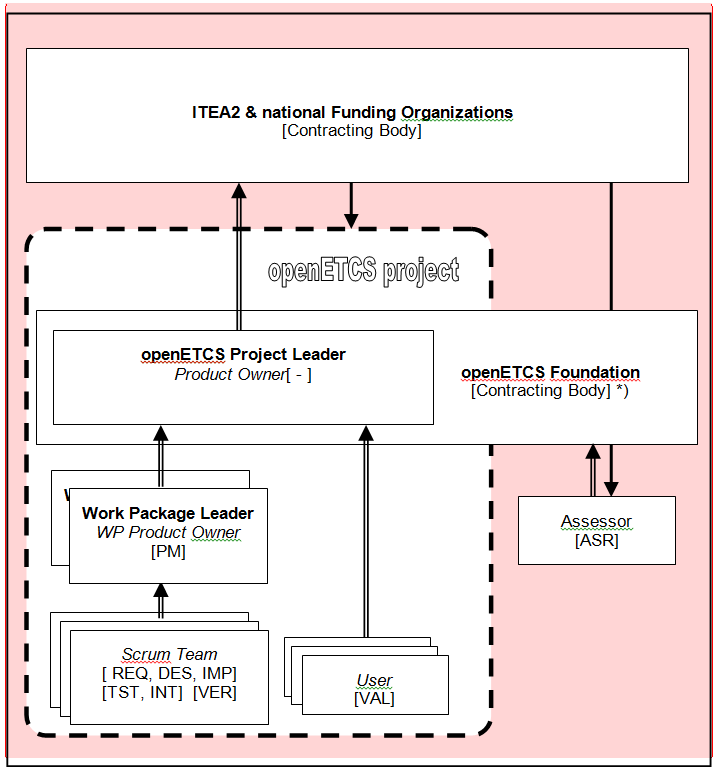
\includegraphics[width=\textwidth]{./figures/organization.PNG}
%\caption{???? Organization ????}
\end{figure}

\textcolor{red}{We need here an explanation to the diagram {\dots}..detailed ???} 

\textcolor{red}{Bernd will deliver content to this part {\dots}.!! }


\section{Life Cycle}
\textcolor{red}{Rico will work on this part!!}

Here we have the understanding of a Project Life Cycle  as well as a Product Life Cycle.

\subsection{Project Life Cycle }
Definition ??? Projects go through six distinct phases. The transitions from phase to phase are open and transparent public reviews.

Connection to 2.2

\begin{figure}
\center
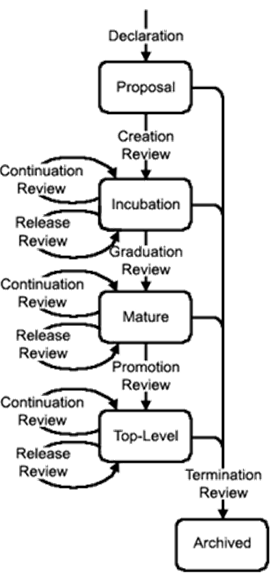
\includegraphics[width=.35\textwidth]{./figures/lifecycle.PNG}
\caption{???? Lifecycle ????}
\end{figure}

\subsection{Product Life Cycle }
Definition 

Here we place : requirements~/~D2.3~/~images~/~\textbf{Process1.png}

Refer To D2.3  the document of marielle  {\dots}. 3  sentences {\dots}  What is the process {\dots}{\dots}.

\subsubsection{?? Open ETCS Software life cycle based on Eclipse in accordance to CENELEC EN50128}
Eclipse Lifecycle has following strategy. It starts in July. It goes for 6 weeks. Within these 6 weeks will have every 2 weeks a Scrum Sprint which means 3 sprints within this 6 weeks. At the end of 6 weeks there will be an interim release. Afterwards the next 6 weeks starts in order to achieve the next interim release. In total we will have 8 times of these 6 weeks. At the end of 8 times each 6 weeks we will have a 4 weeks preparation phase in order to have a proper Major Release. In Total a Major release take one year.  

Now in order to be in compliance with CENELEC, we have to abide by to the rules in Chapter 7 of EN50128 in his lifecycle strategy.


\section{Process}
In framework of Open ETCS project, a Safety certified SIL4 Software has to be supplied, according to the EN50128 standard. The software regarded is the one embedded on the On-Board part of the ETCS system: the EVC.

Development process and its activities are described in this Software Quality Assurance Plan. This document aims at identify, supervise and control all these activities. It provides the quality process and approach needed to avoid developing process hazards, and assures compliancy with the EN50128 requirements.

All documentation delivered in the framework of this software development needs to be compliant with EN 50128 standard (Ref [N01]).


\subsection{Process description}
\textcolor{red}{Jan will evaluate the text below :}

This is the description of the Development Process for the openETCS project. In particular, it describes how participants influence, and collaborate with Projects to achieve these openETCS purposes. The process follows the template of the Eclipse development process\footnote{\url{http://www.eclipse.org/projects/dev\_process/development\_process\_2011.php}}, including minor adaptations.

The openETCS project is a vendor-neutral, open development project supplying methods, methodologies, tools, frameworks, specifications and implementations of ETCS onboard units and related components. openETCS software are extensible in that their functionality is accessible via documented programmatic interfaces. The purpose of the openETCS project, is to advance the creation, evolution, promotion, and support of work products related to openETCS and to cultivate both an open source community and an ecosystem of complementary products, capabilities, and services. 

An Open Source Project needs strong governance because no traditional management structure can be conducted for that. During the last decade there has been an evolution in OSS IT industry. The most important development is ``Eclipse`''. Unfortunately CENELEC is not affected by this evolution. Therefore we need a further development of those requirements by looking into the ``intention and suspected objectives inside CENELEC'' which should be independent from specific legacy styles of management.


\paragraph{Open Source Rules of Engagement}
\begin{description}
\item[Open]openETCS is open and provides the same opportunity to all. Everyone participates with the same rules; there are no rules to exclude any potential contributors which include, of course, direct competitors in the marketplace.

\item[Transparent]Project discussions, minutes, deliberations, project plans, plans for new features, and other artifacts are open, public, and easily accessible.

\item[Meritocracy]openETCS is a meritocracy. The more you contribute the more responsibility you will earn. Leadership roles in openETCS are also merit-based and earned by peer acclaim.
\end{description}

\paragraph{openETCS Ecosystem}
openETCS is the sum of its parts (all of the Projects), and Projects should strive for the highest possible quality in documents, extensible frameworks, exemplary tools, transparent processes, and project openness.

It is the responsibility of the project participants to ...cultivate...an ecosystem of complementary products, capabilities, and services.... It is therefore a key principle that the openETCS Development Process ensures that the projects are managed for the benefit of both the open source community and the ecosystem members. To this end, all openETCS projects are required to:

\begin{enumerate}
\item communicate their project plans and plans for new features (major and minor) in a timely, open and transparent manner;

\item create high-quality and understandable documents, which follow standards and common vocabulary 

\item create platform quality frameworks capable of supporting the building of commercial grade products on top of them; and

\item ship extensible, exemplary tools which help enable a broad community of users.
\end{enumerate}


\paragraph{Clear, Concise, and Evolving}
It is an explicit goal of the Development Process to be as clear and concise as possible so as to help the Project teams navigate the complexities, avoid the pitfalls, and become successful as quickly as possible.

This document imposes requirements and constraints on the operation of the Projects, and it does so on behalf of the openETCS community. It is an explicit goal of the Development Process to provide as much freedom and autonomy to the Projects as possible while ensuring the collective qualities benefit the entire openETCS community.

Similarly, this document should not place undue constraints on Project Leads, the Project Management Board (PMB) or committers that prevent them from governing the process as necessary. We cannot foresee all circumstances and as such should be cautious of being overly prescriptive and/or requiring certain fixed metrics.

The frameworks, documents, specifications, tools, projects, processes, community, and even the definition of Quality continues to, and will continue to, evolve. Creating rules or processes that force a static snapshot of any of these is detrimental to the health, growth, and ecosystem impact of openETCS.

Part of the strength of this document is in what it does not say, and thus opens for community definition through convention, guidelines, and public consultation. A document with too much structure becomes too rigid and prevents the kind of innovation and change we desire for openETCS. In areas where this document is vague, we expect the Projects and all participants to engage the community-at-large to clarify the current norms and expectations.


\subsubsection{openETCS Process Definition}
\textcolor{red}{Jan will evaluate the text below:}

The following describes the guiding principles used in developing this Development Process.

In this document we will describe what exactly are the minimum requirements of CENELEC and how we can conduct them in openETCS project.

\textcolor{red}{Jan will deliver content to this !!!!!!!!}


\subsection{Roles}
\subsubsection[Open Source Roles]{Open Source Roles}
\textcolor{red}{Bernd will contribute !!!} 

Short text : definition of theses 3 roles

Reference of detail description ..

Technical explanation ...clear definition of process .... 

Essential to the Purposes of openETCS is the development of three inter-related communities around each Project:

Contributors and Committers - a thriving, diverse and active community of developers is the key component of any openETCS Project. Ideally, this community should be an open, transparent, inclusive, and diverse community of Committers and (non-Committer) Contributors. Attracting new Contributors and Committers to an open source project is time consuming and requires active recruiting, not just passive ``openness''. The Project Leadership must make reasonable efforts to encourage and nurture promising new Contributors.

Projects must have diversity goals to ensure diversity of thought and avoid relying on any one company or organization. At the same time, we acknowledge that enforcing a particular diversity metric is a poor way to achieve these goals; rather we expect the project leadership to help the diversity evolve organically.

Diversity is a means to an end, not an end in itself, thus diversity goals will differ by project based on the other accomplishments of the project(s).

Projects are required to explain their diversity efforts and accomplishments during Reviews.

Users - an active and engaged user community is proof-positive that the Project{\textquotesingle}s exemplary tools are useful and needed. Furthermore, a large user community is one of the key factors in creating a viable ecosystem around an openETCS project, thus encouraging additional open source and commercial organizations to participate. Like all good things, a user community takes time and effort to bring to fruition, but once established is typically self-sustaining.

Adopters - an active and engaged adopter developer community is the only way to prove that an openETCS project is providing extensible frameworks and extensible tools accessible via documented APIs. Reuse of the frameworks within the companies that are contributing to the project is necessary, but not sufficient to demonstrate an adopter community. Again, creating, encouraging, and nurturing an adopter community outside of the Project{\textquotesingle}s developers takes time, energy, and creativity by the Project Leadership, but is essential to the Project{\textquotesingle}s long-term open source success.

The openETCS community considers the absence of any one or more of these communities as proof that the Project is not sufficiently open, transparent, and inviting, and/or that it has emphasized tools at the expense of extensible frameworks or vice versa.



Definition of roles

User and competencies

Contributer and competencies

Commiter and competencies


\paragraph{??????????Committers Competencies???????}
\textcolor{red}{Bernd will contribute !!!}

According to the EN50128 Standard, all personnel who have responsibilities for the software are organized, empowered and capable of fulfilling their responsibilities. Moreover, these people shall be competent to discharge those responsibilities by demonstrating the ability to perform relevant tasks correctly, efficiently and consistently to a high quality and under varying conditions.

As many committers and contributors are involved in the Open ETCS Project, the people responsible or involved in a project task defined as Key Software Role, have to prove that he has the needed skills to perform this task in accordance with the CENELEC requirements. Indeed, this personnel assigned to the roles involved in the development or maintenance of the software shall be named and recorded.

Therefore, this chapter encompasses 3 different parts:
\begin{itemize}
\item The Needed Competencies Matrix. Based on the Open ETCS Work Packages / Tasks structure, this table describes which competencies are needed for each stake holder depending on its role according to the standard.
\item The Actual Competencies Matrix. Still based on the Open ETCS Work Packages / Tasks structure, this table summarizes the actual competencies of each stake-holder.
\item Deduced from the 2 previous competencies, a Training Plan for Project Stake Holders is defined. This plan aims at allow people responsible for EN50128 compliant activities, to reach the skill and competencies level required for EN50128 standard compliancy.
\end{itemize}


\subsubsection{CENELEC Roles}
\textcolor{red}{Here will Merlin contribute !!!}

Categories..??

Reference to a document which will deliver some information in this regard ??


\subsubsection{Required Competencies Matrix}
Committers will fulfill the required EN 50128 roles! The committer has to deliver her/his qualification!

Contributer does not need to deliver any qualification and does not need to fulfill any competencey

According to CENELEC Requirements, each Committer shall demonstrate their ability to perform relevant Software Key tasks properly, efficiently and consistently to a high quality and under various conditions.

According to CENELEC Requirements, the Task Leaders that are managing software key tasks shall manage these required Competencies for all involved committers. Each competencies and skills needed for each Software Key Role are described in Annex B - Ref [N01].

The Required Competencies Matrix has to be fulfilled by each Task Leader for each Tasks related to a Key Software Role according to the CENELEC requirements. A Matrix template is provided in Annex A.

According to the OpenETCS project structure, all involved committers competencies and skills are summarized in the actual competencies matrix, provided in Ref [N01].

Documented evidence of personnel competence, including technical knowledge, qualifications, relevant experience and appropriate training, shall be maintained by the supplier{\textquoteright}s organization in order to demonstrate appropriate safety organization and accordance to the CENELEC requirements. This documentation activity has to be managed and supervised by the relevant appropriate task leader.


This paragraph describes different quality assurance related documents that have to be issued within each Work Package and task of the project.


\paragraph{Matrix of Competencies according Development Process ?? to CENELEC ..EN50128 and EU Roles \& Rules ???}
\textcolor{red}{Content from Merlin!!!}


\subsubsection{SCRUM Roles}
\textcolor{red}{Bernd will contribute !!!}

openETCS product owner role is fulfilled by the project lead of the EUPL openETCS project. As a product owner of openETCS, he is responsible for the openETCS product backlog.

The project is organized in a hierarchical manner. The project openETCS is split into work packages,. Same way the responsibility for the openETCS product is split to the WP leaders. In scrum, the WP leaders act as WP prduct owners for there respective part.

The WP product owner reports to the leader of the openETCS project. The contribution of all work packages builds the openETCS project.

The role of a workspace product owner nicely fits to the role of a project manager in the sense of EN50128.

Software development is done in Scrum teams. The team as a whole is responsible to reach the sprint targets and put all items to ``Done''. In each sprint, each of the Scrum Teams have to offer (or build) all necessary competences. The contribution of team members corresponds to the CENELEC roles ``Requirement Manager'' [RQM], ``Designer'' [DES], ``Implementer'' [IMP], ``Tester'' [TST], ``Integrator'' [INT] and ``Verifier'' [VER]. Teams need to take care competences for these roles are represented by the team members. However, during lifetime of the project, all team members may act in the different roles. 

In order not to jeopardize quality, we post the limitation an individual is not supposed to proof quality (i.e., review) of his own work. 

In practice, we request for each sprint a person shall not work in  the roles \{RQM, DES, IMP\} on one side and \{VER, INT, TST\} on the other side. 

Besides this restriction every member of the Scrum team can act in any of the roles provided by the team. Acting in various roles increases the competences of the teams over time and, at the same time, also quality and efficiency of team members.

According to CENELEC, the Validator [VAL] has a special responsibility. In our Scrum approach we use the role of the User to fulfill the Validator requirement.The role of the User is an essential component in scrum. In openETCS, naturally, the work packages product owner have to  act as User where appropriate.  In addition, active participation of representatives of the railway owners is required.

In practice, to fulfill the CENELEG Validator point of view, the User has to participate in Sprint Demonstrations and has to have a formal view on the quality aspects for the item. The User is invited also to have a closer look on the daily work of the Scrum teams.

Each Scrum team is supported by a scrum master. The scrum master represents the team at the work package product owner.

The Scrum Team size is recommended to be 6 members + scrum master.


\paragraph{Sprints in openETCS Scrum}
\textcolor{red}{Bernd will contribute !!!}

The schedule of the project is organized in sprints. Sprint, in general take 2 or 3 weeks of time. The frame schedule of the sprints will be defined by the openETCS product Owner and has to be aligned with eclipse release planning. Where necessary the sprint plans of different work packages might be synchronized, e.g., between Tools and the tool users. The project makes use of regular (weekly) Scrum of Scrum meetings. These meetings are meant to plan and improve the interaction of the work packages and to manage impediments.

Inside work packages the Work Package Product Owner is responsible for organizing Sprint Planning meetings, Sprint Review meetings and Sprint Retrospective according to Scrum.

The Scrum Master calls for a daily scrum meeting and represents the team in other activities.

Teams are responsible to complete all parts of implementation of their committed tasks. The result has to be documented at the end of the sprint in the sprint review for each item ``Done'' in the sprint. ``Done'' criteria are to be defined for each item in the sprint planning.

\paragraph{The Backlogs in openETCS Project}
\textcolor{red}{Bernd will contribute !!!}

The work in openETCS is split into several work packages. In general, the tasks of each work package build the work package backlog. 

The openETCS backlog defines priority of features for the project as a whole, i.e., workspace backlogs have to follow the priority of the project.

The priority of items in the backlogs is visible by the sequence in the backlog.

Items for daily work are managed in the task backlogs for the Scrum Teams. The backlogs are filled before starting the sprint in the sprint planning meeting. At sprint end the sprint result has to be reported back to the product backlog. This is one of the topics of the sprint review. 

The use of a professional backlog tool is highly recommended. The evaluation and selection of a tool is in responsibility of the project office. 


\paragraph{The role of the Assessor in openETCS}
\textcolor{red}{Bernd will contribute !!!}

In order to make the openETCS results easier useable by the industry after our initial project has finished the role of the Assessor [ASR] has to be implemented as an independently acting personality. With this role we follow the CENELEG proposal. We propose to use the openETCS foundation as a contractor for the Assessor. The Assessor will report to the openETCS foundation and, in the special situation of this ITEA 2 project, to ITEA 2.


\subsection{Documentation}
\textcolor{red}{Rico will work on this !!}

\subsubsection{Documentation Structure}

\paragraph{Document Labeling and owner}
Document Labeling

Refer to labeling document {\dots}..from Baro 

Templates , document organization and shape 

Reference ot the templates ??

Contribution from Baro ????


\paragraph{Overview Documents ..???}
\textcolor{red}{Jan will deliver here !!}

WP structure

Connection between WPs

Document Owner {\dots}.Jan will here contribute !! 

Following Plans will enhance the quality of openETCS project and some of them are highly recommended in CENELECT Ref [N01].

\begin{itemize}
\item Software Configuration management Plan
\item Maintenance Plan
\item Validation Plan
\item Verification Plan
\item System Testing plan  
\item Implementation Plan
\item Software deployment Plan
\item Training Plan
\end{itemize}


\paragraph{Terminology}
Refer to terminology database

Reference use terminology for documents {\dots} 

\textcolor{red}{Jan will contribute here !!}


\paragraph{Organizations and Logos in Documentation}
\textcolor{red}{Rico will work on this !!}

The logo of such organization like ITEA2 has to be considered in openETCS Documentation. On front page as well as certain other places an evaluation is needed to find out which logos, from which organization. On one side we have to consider the permission issue and on the other side we have to show the appreciation on every type of participation. 


\paragraph{IP Clean}
\textcolor{red}{Rico will work on this !!}

How do we deal with License scenario/handling? 

One of the major subjects in openETCS is, IP (INTELECTUAL PROPERTY) and all openETCS partners have to work IP clean.


IP Clean means: A Citation, a Text or a Diagram which belongs to somebody else is allowed to be mentioned or used in a Document just with the permission of the owner in writing. Otherwise it has to be just a reference to that IP subject.


\subsubsection{Documentation Control}

\paragraph{Checking and Approval}
\textcolor{red}{Jan and Bernd will raise this part at Friday meetings!!}

The idea/review process of S.Baro has to be placed here {\dots}{\dots} in an exel document

Refer to a document for review details {\dots}which describes the Github review procedure from Bernd !!

A short explanation of next 5 points {\dots}

Regarding release and approval of the document, refer to an additional document 

The quality assurance activities, actions and documents shall be specified or referenced in this document. A Software Quality Assurance Verification Report shall be written, under the responsibility of the Verifier, on the basis of all the input documents available from the project.

For each document issue, an inspection process shall be realized according to the following steps:
\begin{itemize}
\item A first draft version of the document is written by a person part of the relevant task committers;
\item Then, another person, competent and independent from the author, will review the document through a revision sheet encompassing all the remarks gathered during the document review;
\item Once the review phase done, the revision sheet is sent to the author, who considers or not the remarks, and justifies their acceptance or refusal;
\item Once the document has been updated by the author, the document has to be sent back to the reviewer, in order that he checks the remarks acceptance or refusal, and their justification. If the author{\textquoteright}s answers are to be discussed again;
\item The document can be issued in an official version and distributed once all remarks have been closed.
\end{itemize}
The document author shall establish, document and maintain procedures for control of the external suppliers, including methods and relevant records to ensure that the requirements provided to the External Customer are adequate and complete.

\paragraph{Document Dissemination }
\textcolor{red}{Rico will contribute!!}

How do we use sharepoint?

How do we work on GitHub?

\paragraph{Documentation Archiving}
Explanation how all documents will be archived {\dots}. Rico will contribute!!


\subsubsection{Tracking and tracing of deviation}
\textcolor{red}{Rico will contribute!! Getting advice from Jastram.}

An Introduction here !!

In order to comply with a SIL4 level according to the CENELEC standard, the following requirements have to be respected: {\S}6.5.4.5, {\S}6.1.4.5, {\S}6.2.4.13, {\S}7.7.4.8, {\S}7.7.4.10.


\paragraph{Traceability}
\textcolor{red}{Rico will contribute!! Getting advice from Jastram.}

A definition. 

We need here a relevant explanation to openETCS???

Definition of technical process in Tools! 

Could jastram be the right person to this subject?

Tool chain?

In order to comply with a SIL4 level according to the CENELEC standard, the following requirements have to be respected: {\S}5.3.2.8, {\S}5.3.2.9, {\S}5.3.2.10, {\S}5.3.2.13, {\S}5.3.2.14.

Following content needs to be evaluated !!

According to EN50128 Standard, the Traceability to requirements shall be an important consideration in the validation of a safety-related system and means shall be provided to allow this to be demonstrated throughout all phases of the lifecycle.

Within the context of this European Standard, and to a degree appropriate to the specified software safety integrity level, traceability shall particularly address:

\begin{itemize}
\item traceability of requirements to the design or other objects which fulfill them,
\item traceability of design objects to the implementation objects which instantiate them,
\item Traceability of requirements and design objects to the tests (component, integration, overall test) and analyses that verify them.
\end{itemize}
The overall traceability and documentation requirements are detailed in the Configuration Management plan (ref [{\dots}]).


\paragraph{Configuration management}
\textcolor{red}{Rico will contribute!! Getting support from Alstom and advice from SQS!}

Here the definition has to be more relevant to openETCS {\dots}
Short explanation Rico will contribute ..( 3.18 can be used here) and reference to a document which is coming from ALSTOM !!

Following content has to be evaluated:

Description of the used SW 



\begin{flushleft}

\begin{tabular}{|m{3cm}|m{11cm}|}
\hline
\rowcolor{myblue}
\multicolumn{2}{|c|}{CMS Tool} \\\hline
Name &
Git \\\hline
Manufacturer &
free software initially designed and developed by Linus Torvalds and distributed under the terms of the GNU General Public License\\\hline
Version &
1.8.0.2 for windows\\\hline
Characteristics &
Web-based revision control hosting service for software development and code sharing (http://git-scm.com/)

Distributed Version Control System

Compatibility with existing systems/protocols (Subversion, Bugtracker,...)\\\hline
Functions &
fully mirror of the repository

Incremental development: ``patches'', changelogs etc

Provenance tracking: shows who did what, when is built in to a revisioning system

Broader participation: changes can be reverted.

Peer-2-peer model: different contributors can work simultaneously and independently (Distributed). Extra ``features'' can added independently of mainline development with re-integration later. 

supports rapid branching and merging, and includes specific tools for visualizing and navigating a non-linear development history\\\hline
\end{tabular}
\end{flushleft}


Description of how data is been archived and versioned

During the OpenETCS project will be used Scrum methodology. Scrum is an iterative, incremental framework for projects and products or application development. It structures development in cycles of work called Sprints. These iterations are short in time, no more than one month each, and take place one after the other without pause. 

At the beginning the SCMP will be developed. In this plan all project SCIs will be identified to ensure that the items are properly stored for traceability, and procedures for placing configuration items under software configuration management by means of the definition of a hierarchical directory structure will be established and identification scheme for the components to uniquely identify each individual component will be create. A proper configuration identification schema identifies each component of the system and provides traceability between the component and its configuration status information.

During the Sprint selects items from a prioritized list, these items will be under configuration management and will be detailed in the configuration management plan (SCMP). 

Every day the team gathers briefly to inspect its progress, and adjust the next steps needed to complete the work remaining. At the end of the Sprint, the team reviews the Sprint, and demonstrates what it has built. 

The team commits to complete the items by the end of a Sprint.

Every finished CI of Sprint will be tagged, with this OpenETCS will have a stable version of every CI.

This way of working will produce a huge number of versions of configuration items, these versions will be controlled using Git tool. OpenETCS has a really concrete WP (SRS, Model-Code, Safety and Validation and Verification). These WPs are in closed communication among each other, but their working schedule has different speed, so the versions of the CI of one WP could not match with the versions of related CIs of other WPs. Due to this, it was decided to define Baselines of each WP.

Product development

OpenETCS team goal is having a complete control of the final product developed and assure the quality of the product, following the requirements specify. In order to achieve this objective a configuration process has been defined. This process has established 6 different baselines: SRS, Model/Code, Safety, V\&V, Product and Archived baselines. 

The baselines describe the functional and physical attributes of these CIs, in order to maintain control of changes occurring to existing items and new {\textquoteleft}{\textquoteleft}enditems{\textquoteright}{\textquoteright} or deliverables within the projects. The project processes result in establishing approved baselines and related descriptions in a timely manner. 

SCMP will set when a baseline will be created. The creation of a baseline will depend on the status of the CIs and its versions.


Definition of each baseline:
\begin{description}
\item[SRS baseline] will contain the specific version of the components requirements and the supported tools
\item[Model/Code baseline] will be created as soon as it is consider that concrete code and model version could be integrated. This baseline will also contain the supported tools to create the models, code and so on.
\item[Safety baseline] will contain the specific version of documentation of the safety items, as well as, the required tools for granting the safety of the project. 
\item[V\&V baseline] will contain the supported tools for testing, as well as the test cases, use cases, test data, test environment and the whole stuff required to assure the quality of the project and product.
\item[Product baseline] will integrate all the different baseline of the WPs to create de tagged release of the product, as well as, any other software or documentation that is needed for the release of the product.
\item[Archived baseline] will contain the back-up of the project. 
\end{description}

CCB will have the authority to approve and make changes to the components of Product baseline and every WP leaders will be able to make changes in their own baseline.

Any changes from the baselines are documented because they affect unique items. The baselines reflect the differences from the ``as planned'' through ``as released''.

All the plans are not going to be part of the baselines; they are going to be reviewed periodically.

Granting the whole management configuration system

In order to grant the management of this system, Configuration Audits will be carried out. Periodically, the configuration status information will be reviewed to verify its accuracy and completeness.  The CCB will identify the configuration reviews to be performed. The list of configuration reviews and procedures are detailed in the SCMP. Reviews will analyze and note any discrepancies between the configuration status information and the current situation.

With the establishment of the Configuration Audits it is going to maintain the traceability among all configuration items (requirements, model and code, software tools and documentation of the project, etc.). Doing this, the traceability becomes part of the Configuration Management and will allow as to have a global view of the whole system and control for the analysis of the risk impact.


Finally a Version description document (VDD) will be created in order to summarize the content of the version and maintain the traceability among the baselines.

Description how accessing rights are managed and administrated

The members of the projects that are involved in each item (source, document, plans, software, tools and so on) will have accessed and writing rights them. It will not be access to every item by every members of the project. This access will be controlled using Git tool.



{\textbullet}\ \ Version control management

The WP leader will identify the specific CI personnel responsible of doing the version.



{\textbullet}\ \ Baseline control management

At WP level, baseline control will be more decentralized.  A component baseline will be established for each CI that will capture the operational parameters with which that component was evaluated and deployed.  Any changes to this baseline must be approved by the specific WP leader and documented by the person who makes the changes. A larger number of people will be able to make changes. The WP leader will identify the specific CI personnel authorized to make changes and the specific changes that each person is authorized to make. Typically these changes will not require CCB approval, but periodic configuration reviews will enable the CCB to monitor CI level changes and refine the process in case it is necessary.


{\textbullet}\ \ Product baseline control management

At product level, baseline control will be centralized at the CCB. This will prevent significant system changes from being performed before all affected organizations have been informed and have provided their input.


\begin{tabular}{|m{3cm}|m{11cm}|}
\hline
\rowcolor{myblue}
\multicolumn{2}{|c|}{Scope}\\\hline
Stand Alone &
The bug or change request mainly affects one phase of the life-cycle (e.g erroneous development of the activities of a phase)\\\hline
Cross-institutional &
The bug or the change request has an impact on different phases of the development life-cycle (e.g missing or erroneous specification).\\\hline
\end{tabular}

\begin{flushleft}
\begin{tabular}{|m{3.5cm}|m{10.5cm}|}
\hline
\rowcolor{myblue}
\multicolumn{2}{|c|}{Location of the error; part(s) of the system affected by the error, CIs, versions,...}\\\hline
Software &
Details to complete\\\hline
Formal specification &
Details to complete\\\hline
Model &
Details to complete\\\hline
Documentation &
Details to complete\\\hline
Others &
Details to complete\\\hline
\end{tabular}
\end{flushleft}


\begin{flushleft}
\begin{tabular}{|m{3cm}|m{11cm}|}
\hline
\rowcolor{myblue}
\multicolumn{2}{|c|}{Severity}\\\hline
Critical &
The bug causes a failure of the complete software system, subsystem or a program within the system\\\hline
High &
The bug does not cause a failure, but causes the system to produce incorrect, incomplete, inconsistent results or impairs the system usability.\\\hline
Medium &
The bug does not cause a failure, does not impair usability, and does not interfere in the fluent work of the system and programs.\\\hline
Low &
The bug is an aesthetic, is an enhancement or is a result of non-conformance to a standard. \\\hline
\end{tabular}
\end{flushleft}


\begin{flushleft}
\begin{tabular}{|m{3cm}|m{11cm}|}
\hline
\rowcolor{myblue}
\multicolumn{2}{|c|}{Priority}\\\hline
Immediate &
The bug or the change request should be resolved immediately\\\hline
High &
This bug or the change request should be resolved as soon as possible in the normal course of development activity, before the software is released. \\\hline
Medium &
This bug or the change request should be repaired after serious bugs or emergency change requests have been fixed. \\\hline
Low &
It can be resolved in a future major system revision or not be resolved at all.\\\hline
\end{tabular}
\end{flushleft}


\begin{flushleft}
\begin{tabular}{|m{3cm}|m{11cm}|}
\hline
\rowcolor{myblue}
\multicolumn{2}{|c|}{Classification}\\\hline
Bug &
To complete\\\hline
Enhancement &
To complete\\\hline
New Requirements &
To complete\\\hline
Change &
To complete\\\hline
\end{tabular}
\end{flushleft}

The receiving parties will assess the impact of the Problem/Change Request. Depending on the scope of the request, the PM will engage all or only some of the members of the Project Expert Team. A Testing (V\&V) expert will always be engaged. The integration of the CMIS and the Bug tracker Tool will help the Team in performing a proper impact assessment. 


The individual impact assessments (IA) will be registered in the Bug tracker Tool, compiled and analysed by the PM:

\begin{itemize}
\item In case of change requests with a clear cross-institutional impact, the impact assessment (IA) will be submitted to the CCB for approval.
\item In the case of bugs or minor change requests, the IA will be assessed by the PM. In case the impact is acceptable, it will be sent to the appropriate party for its implementation.
\begin{itemize}
\item The implementation plan will be attached to the problem/change request in electronic format. The implementation plan will include both implementation and verification/validation tasks.
\item As the implementation is performed, 
\begin{itemize}
\item the identification code of the problem/change request will be referenced in the configuration items as they are modified, 
\item the Bug tracker Tool will register the details (CI, scope) of the problem resolutions activities performed
\end{itemize}
\item As soon as the implementation plan is finalised, the status of the Problem/Change Request will be {\textquotedblleft}Fixed{\textquotedblright} and therefore ready for auditing.
\item The implementation will be audited by the SQA and the issue will become either closed or re-open
\end{itemize}
\item In case the Problem/Change request is not accepted, the PM will include the reason in the Bug tracker Tool and the issue will be closed. 
\end{itemize}


The SQA will perform periodical audits and quality assessments of the bugs and change requests received. 

\begin{itemize}
\item Audits to verify the process itself.
\item Quality Assessments to verify the evolution of the product quality. 
\end{itemize}

 
\begin{figure}
\centering
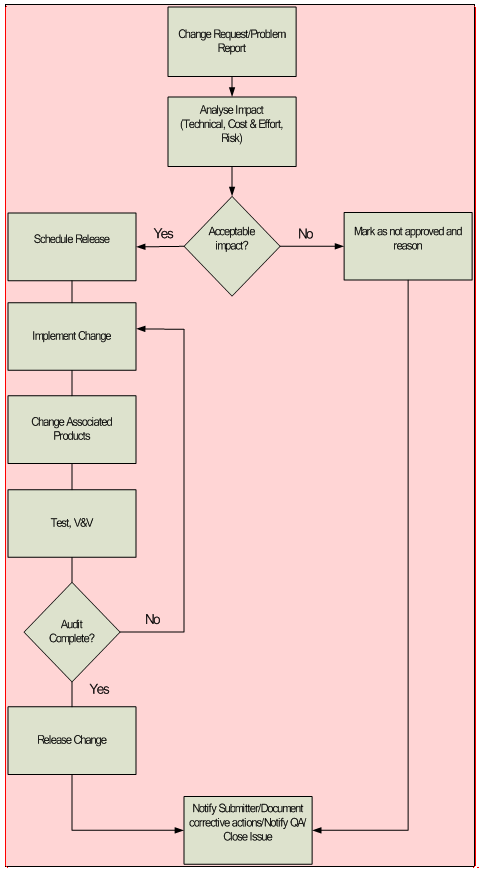
\includegraphics[scale=1.3]{./figures/changerequest.PNG}
\caption{Change/Problem Request process}
\end{figure}


\begin{flushleft}
\tablefirsthead{}
\tablehead{}
\tabletail{}
\tablelasttail{}
\begin{supertabular}{|m{5cm}|m{9cm}|}
\hline
\rowcolor{myblue}
Role &
Responsibility\\\hline
Project Manager &
Development of the Software Deployment Plan

Monitoring and Approval of the software implementation\\\hline
Configuration Management Staff &
Build the product/software release, run regression tests, perform configuration audits and accounting, baseline and packaging the release.

Complete traceability including destination of the software.\\\hline
Implementation Team &
Preparation of the Version Description Document

Preparation of the Software Implementation Manual

Elaboration of the Software implementation Records\\\hline
Verifier &
Preparation of the Deployment Verification Report\\\hline
Quality Assurance Manager &
Independent reviewer of both the processes and the corresponding outcomes\\\hline
\end{supertabular}
\end{flushleft}



\begin{flushleft}
\tablefirsthead{}
\tablehead{}
\tabletail{}
\tablelasttail{}
\begin{supertabular}{|m{7cm}|m{7cm}|}
\hline
\rowcolor{myblue}
Quality mechanisms for Safe deployment &
Technique \& Approach\\\hline
Software Self-identification Mechanisms

(9.1.4.11) &
~
\\\hline
Error detection and/or avoidance mechanisms during deployment process (store, transfer, transmission and/or duplication of code operations)

(9.1.4.20) &
~
\\\hline
Automatic detection and safe management of incompatible components/versions

(9.1.4.8, 9.1.4.9) &
~
\\\hline
Provision of appropriate and accurate diagnostic information &
~
\\\hline
Safe Roll back capabilities  &
~
\\\hline
\end{supertabular}
\end{flushleft}


\begin{flushleft}
\tablefirsthead{}
\tablehead{}
\tabletail{}
\tablelasttail{}
\begin{supertabular}{|m{5cm}|m{9cm}|}
\hline
\rowcolor{myblue}
Role &
Responsibility\\\hline
Project Manager/Maintenance Manager (if different) &
Development of the Software Maintenance Plan

Preparation and maintenance of the project history register (already started at the beginning of the project)

Responsible for the Impact Assessment processes

Preparation of the software maintenance reports\\\hline
Configuration Management Staff &
Maintain complete software (CI) maintenance registers and complete and accurate modification reports\\\hline
CCB &
Approval of changes\\\hline
Implementation Team &
Implementation of changes

(as during the development process)\\\hline
Verifier

~
 &
Preparation of the software maintenance verification report

Verification activities, as during the development process\\\hline
Validator &
Validation activities, as during the development process\\\hline
Quality Assurance Manager &
Independent review processes\\\hline
\end{supertabular}
\end{flushleft}


\begin{flushleft}
\tablefirsthead{}
\tablehead{}
\tabletail{}
\tablelasttail{}
\begin{supertabular}{|m{7cm}|m{7cm}|}
\hline
\rowcolor{myblue}
Quality mechanisms for Maintainability &
Technique \& Approach\\\hline
Coding Standards &
~
\\\hline
Impact Assessment &
Before each implementation\\\hline
Data register and analysis &
Creation and maintenance of a project history register\\\hline
Design method selection mechanisms to facility the maintainability (7.3.4.28) &
~
\\\hline
Attenuation actions mechanisms (9.2.4.20) &
~
\\\hline
Mechanisms for evaluating the appropriateness of the methods, tools and techniques used in the modification/maintainability (part of 9.2.4.2 and CENELEC 126 phase 13) &
~
\\\hline
SW description mechanisms (7.1.1.1) &
~
\\\hline
Control mechanisms to guarantee the corrective actions adoption (6.6.4.1) &
~
\\\hline
Provision of appropriate and accurate modification management system (6.6.4.1) and configuration management system (6.5.4.12) &
~
\\\hline
\end{supertabular}
\end{flushleft}









\paragraph{Fault Management}
Here the definition has to be more relevant to openETCS {\dots}{\dots}..SQS ??? 

\textcolor{red}{Rico will contribute!! Getting advice from Jonas.}

\textcolor{red}{A Document is needed advice from Bernd}



\paragraph{Grievance Handling}
A platform is needed to handle different cases of Grievance as well as problem reporting and during the development phase the ticketing of problem records between the development team and test team.
Failures and errors encountered during the review activities (QA. Verification, Validation, Assessment) planned in the software development life-cycle, problems reported by users and customers as well as change requests initiated by any of the system stakeholders will be reported and managed through the Bugtracker.NET Tool. This tool will be integrated with the CMIS and will be configured to implement and record all the information generated during the process.

The integration with the CMIS will permit:
\begin{itemize}
\item Traceability between Change/Problem Requests and the configuration items where the problem was located.
\item Traceability between the configuration items modified and the corresponding Change/problem request. 
\end{itemize}
The implementation of the workflow will permit:
\begin{itemize}
\item A complete history trail of the Change/Problem Request
\end{itemize}

The process will be as follows:

Problem and Change requests (see appendix A for template) will be collected via web and notified to both the Project Manager (PM) and the Quality Manager (QM) as soon as they are received. The Project Manager will perform a first review (completeness, accuracy, scope, severity, priority, classification) of the information provided and will re-direct the request to the relevant parties within the Project Expert Team for further analysis and/or implementation. If needed, additional information will be requested. All the information provided will be attached to the Problem/Change Request in electronic format. The Problem/Change request will be assigned a unique Id. Code, and will be assigned the status of ``Open''.


\subsubsection{Methods, measures and tools for quality assurance}
\textcolor{red}{Rico will contribute!! Getting advice from S.Baro and Marielle!!}

Short definition, {\dots} asking S.Baro and Marielle for contribution {\dots}..There is a document from marielle 

Objective : which tools and methods have been chosen according to each phase of software life cycle !!

How do we deal with coding standards ????????

All Methods, measures, use of tools and overall requirements for a SIL4 quality assurance are given in Annex A.3 - Ref [N01]

This chapter is structured according to the Software lifecycle phases. (See This document 2.4.4). The Details of methods, measures, tools, and the Overall Software Test Specification will be precisely described in the V\&V plan (Ref [{\dots}.]).

The structure of Documentation has to be defined here. We have to analyze and follow the way and approach of Eclipse Documentation. 


\subsubsection{Justification of chosen Tools and Methods}
\textcolor{red}{Rico will contribute!! Getting advice from S.Baro and Marielle!!}

We have to refer here to 2 Documents !!

Explanation and justification on, why we chose existing tools and methods and why they are compliant to SIL4 scenario {\dots}.



\subsubsection{Software Maintenance}
\textcolor{red}{Rico will write 3 sentences {\dots}process? WP2 and management ?}

Process Definition see [N1 -- Chapter 9.2]

[F0E0?] additional project specific tasks


\subsubsection{Software Deployment}
\textcolor{red}{Rico will contribute : Refer to FPP}

Process Definition see [N1 -- Chapter 9.1]

[F0E0?] additional project specific tasks



\subsection{System Testing V\&V ?????????? }
\textcolor{red}{Jan has to please tell us his view!! WP4 advice!!}
Refer to the Document V\&V plan, accountability on WP4 !!

Explanation (short)  {\dots}.from Jan or Marc and a reference to V\&V plan {\dots}.


\subsection{Tool Chain Quality Assurance}
\textcolor{red}{Rico has to coordinate in order to get this part sorted be Michael jastram}

We have to involve WP7 and Michael Jastram in this.

Whithin the Toolchain we have to ensure the co-operation {\dots} 

Refer to 3 Documents

O7.3.1 Tool chain development plan (or equivalent) Sep-2013 T0+15 no

O7.3.2 Specification of tool interoperability mechanisms

O7.3.3 Guideline for developing the tool chain according to CELENEC



\subsection[Toolchain deployment and Maintenance]{Toolchain deployment and Maintenance}
\textcolor{red}{Rico has to coordinate : Jonas and Michal has to give here their Input.}


\subsection{Requirements for certification \& Management of Graduated Projects}
\textcolor{red}{Merlin will deliver here !!}

Refer to Merlins Document D2.2 {\dots}..

Michael Jastram will deliver some input {\dots}


\section{References and Abbreviation}
\textcolor{red}{Peter will work on this part !!}

\subsection{Referenced Standards, Directives and Regulations}

\begin{flushleft}
\tablefirsthead{\hline
\rowcolor{myblue}
Nr. &
Document &
\centering\arraybslash Edition\\}
\tablehead{\hline
\rowcolor{myblue}
Nr. &
Document &
\centering\arraybslash Edition\\}
\tabletail{}
\tablelasttail{}
\begin{tabular}{|m{1cm}|m{10cm}|m{3cm}|}
\hline
\rowcolor{myblue}
Nr. &
Document &
\centering\arraybslash Edition\\\hline

[N01] &
EN 50128 Railway applications -  Communication, signalling and processing systems -  Software for railway control and protection systems &
\centering\arraybslash 2011-06\\\hline
[N02] &
EN 50126 Railway applications - The specification and demonstraticn of Reliability, Availability, Maintainability and Safety (RAMS) &
\centering\arraybslash 2000-03\\\hline
[N03] &
EN 50129 Railway applications --  Communication, signalling and processing systems --  Safety related electronic systems for signalling &
\centering\arraybslash 2003-12\\\hline
[N04] &
EN~61508 Functional safety of electrical/electronic/programmable electronic safety-related systems &
{\centering 2010\par}

\centering\arraybslash Edition 2.0\\\hline
[N05] &
2008/57/EC -- Interoperability Directive &
\centering\arraybslash 17.06.2008\\\hline
[N06] &
2011/18/EU -- Interoperability Directive (change of annexes) &
\centering\arraybslash 01.03.2011\\\hline
[N07] &
2012/88/EU -- TSI CCS

technical  specification  for  interoperability  relating  to  the  control-command  and  signalling subsystems  of  the  trans-European  rail  system &
\centering\arraybslash 25.12.2012\\\hline
\end{tabular}
\end{flushleft}



\subsection{Referenced Documents}
\begin{center}
\tablefirsthead{\hline
\rowcolor{myblue}
Doc. Nr.: &
Title &
Date\\}
\tablehead{\hline
Doc. Nr.: &
Title &
Date\\}
\tabletail{}
\tablelasttail{}
\begin{supertabular}{|m{2cm}|m{9cm}|m{3cm}|}
\hline
\centering [D01] &
Full Project Proposal openETCS &
11.04.2012\\\hline
\centering [D02] &
EN50128:2011 &
~
\\\hline
\centering [D03] &
TSI Subset 026 &
~
\\\hline
\centering [D04] &
TSI Subset 036 &
~
\\\hline
\centering [D05] &
TSI Subset 076 &
~
\\\hline
[SCRUM] &
Roman Pichler : Agile Product Management with Scrum &
22.3.2010

~
\\\hline
[SCRUM] &
Ken Schwaber and Mike Beedle : Agile Software Development with Scrum, Pearson Studium &
24.4.2008\\\hline
\centering FM &
Jean-Francois Monin : Understanding Formal Methods


&
17.1.2003\\\hline
\centering [ECLIPSE] &
t.b.d &
~
\\\hline
\end{supertabular}
\end{center}


\subsection{Abbreviations}
\begin{flushleft}
\tablefirsthead{\hline
\rowcolor{myblue}
Abb. &
Meaning\\}
\tablehead{\hline
\rowcolor{myblue}
Abb. &
Meaning\\}
\tabletail{}
\tablelasttail{}
\begin{supertabular}{|m{2cm}|m{12cm}|}
\hline
ASR &
Assessor\\\hline
CCS &
control-command and signalling subsystems  \\\hline
DES &
Designer\\\hline
ERTMS &
European Rail Traffic Management System

Train signaling system equipment based on a single Europe-wide standard for train control and command systems.\\\hline
ERA &
European Railway Agency\\\hline
ETCS &
European Train Control System

It is a signalling, control and train protection system designed to replace the many incompatible safety systems currently used by European railways\\\hline
EUPL &
European Union Public Licence\\\hline
EVC &
European Vital Control\\\hline
GSM-R

(train radio) &
Global System for Mobile Communications - Rail(way)

It is an international wireless communications standard for railway communication and applications.\\\hline
HR &
Highly Recommended\\\hline
HW &
Hardware\\\hline
IMP &
Implementer\\\hline
INT &
Integrator\\\hline
MVB &
Multifunction Vehicle Bus

It is a part of the Train Communication Network (TCN), and it takes part in digital operation in the train. MVB is the bus part in each coach, and the Wire Train Bus (WTB) allows connecting the MVB parts with the train control system.\\\hline
NA &
Not Applicable\\\hline
OBU &
On-Board Unit\\\hline
REQ &
Requirements Manager\\\hline
R\&D &
Research and Development\\\hline
SIL &
Safety Integrity Level\\\hline
SME &
~
\\\hline
SRS &
Software Requirements Specification\\\hline
SW &
Software\\\hline
SW-SIL &
Software-Safety Integrity Level (EN 50128:2011)\\\hline
TSI &
Technical Specification for Interoperability\\\hline
TST &
Tester\\\hline
VAL &
Validator\\\hline
VER &
Verifier\\\hline
V\&V &
Verification and Validation\\\hline
WP &
Work Package\\\hline
ASR &
Assessor\\\hline
ERTMS &
European Rail Traffic Management System

Train signaling system equipment based on a single Europe-wide standard for train control and command systems.\\\hline
ETCS &
European Train Control System

It is a signalling, control and train protection system designed to replace the many incompatible safety systems currently used by European railways\\\hline
GSM-R

(train radio) &
Global System for Mobile Communications - Rail(way)

It is an international wireless communications standard for railway communication and applications.\\\hline
MVB &
Multifunction Vehicle Bus

It is a part of the Train Communication Network (TCN), and takes part in digital operation in the train. MVB is the bus part in each coach, and the Wire Train Bus (WTB) allows connecting the MVB parts with the train control system.\\\hline
SIL &
Safety Integrity Level\\\hline
SW &
Software\\\hline
SW-SIL &
Software-Safety Integrity Level (EN 50128:2011)

~
\\\hline
FM &
Formal Methods\\\hline
IP &
Intellectual Property\\\hline
IP Clean &
No IP without permission in writing \\\hline
~
 &
~
\\\hline
\end{supertabular}
\end{flushleft}


\end{document}
